\documentclass{article}
\usepackage[preprint]{neurips_2026}

\usepackage[utf8]{inputenc}
\usepackage[T1]{fontenc}
\usepackage{hyperref}
\usepackage{url}
\usepackage{booktabs}
\usepackage{amsfonts}
\usepackage{amsmath}
\usepackage{microtype}
\usepackage{xcolor}
\usepackage{graphicx}
\usepackage{float}
\hypersetup{hidelinks}

% This is an ES 678 course paper, not a conference submission.
\makeatletter
\renewcommand{\@noticestring}{ES 678 Course Project}
\makeatother

\title{Do Multi-Domain EEG Features Improve Subject-Level ADHD Classification?}

\author{%
  Aryan Dave \\
  Roll Number: [Enter IITGN Roll Number] \\
  ES 678 \\
  Indian Institute of Technology Gandhinagar
}

\begin{document}
\maketitle

\begin{abstract}
This paper evaluates whether multi-domain EEG features improve subject-level classification of children with attention-deficit/hyperactivity disorder (ADHD) relative to spectral features alone. Using a public dataset of 121 children (61 ADHD and 60 controls), eight EEG channels were segmented into 5,621 epochs. We compared a 40-feature spectral representation with a 199-feature representation combining statistical, spectral, nonlinear, wavelet, fractal, connectivity, and Hjorth features. Logistic Regression, Random Forest, and an RBF-kernel Support Vector Machine (SVM), with a Dummy Classifier baseline, were assessed using five-fold participant-grouped cross-validation. Epoch probabilities were averaged to obtain one prediction per child. The multi-domain representation achieved 77.7\% accuracy for all three learned models; Random Forest obtained the highest ROC-AUC (86.3\%), while SVM obtained the highest ADHD sensitivity (88.5\%). The findings are exploratory and do not establish clinical diagnostic performance.
\end{abstract}

\section{Problem and Motivation}
ADHD assessment relies on clinical information and behavioural evidence. Electroencephalography (EEG) offers a non-invasive recording of brain activity and has been investigated as a source of quantitative features for studying ADHD. The question in this project is whether classical machine-learning models can distinguish children with ADHD from controls using EEG-derived features, and whether a richer feature representation improves generalization to unseen participants. The prediction target is the participant-level ADHD/control label, not the label of an individual time point or epoch. This distinction is important because a single child contributes many correlated EEG observations. Prior studies have explored multi-resolution feature selection and automated classification using pediatric EEG data \citep{attallah2024,alim2023}. The project investigates a potential screening-related signal; it does not propose EEG classification as a substitute for clinical assessment.

\section{Data and Preparation}
We use the ``EEG data for ADHD/Control children'' dataset published through IEEE DataPort (DOI: 10.21227/rzfh-zn36) \citep{nasrabadi2020}. The notebook accessed a CSV mirror distributed through Kaggle \citep{kagglemirror}. The dataset contains 121 children aged 7--12 years (61 ADHD and 60 controls), recorded using 19 EEG channels at 128 Hz during a visual-attention task. The inspected CSV contains 2,166,383 time-point rows and 21 columns (19 channels, class, and participant ID). We selected eight channels: F3, F4, Fz, P3, P4, Pz, O1, and O2.

The supplied implementation formed 5,621 epochs using 256-sample (2-second) windows with a 384-sample (3-second) step, leaving a 1-second gap between successive windows. Each epoch has a participant ID and binary label (ADHD=1, control=0). The spectral subset contains five measurements per channel---theta, alpha and beta power, theta/beta ratio, and theta/alpha ratio---for 40 features. The multi-domain vector contains 24 features per channel (192 total), four connectivity features, and three cross-channel interactions, for 199 features. The per-channel features include statistical moments, spectral measures, Higuchi fractal dimension, entropy, wavelet energies, Katz and Petrosian fractal dimensions, and Hjorth parameters. No additional band-pass filtering, baseline correction, or ICA-based artifact removal is performed by the submitted feature-extraction code; these procedures are therefore not claimed. Non-finite feature values are converted to missing values and median-imputed inside each training pipeline.

\section{Methods}
The baseline is a prior-probability Dummy Classifier. Candidate models are Logistic Regression, Random Forest \citep{breiman2001}, and an RBF-kernel SVM \citep{cortes1995}. The learned-model pipelines apply median imputation and ANOVA \texttt{SelectKBest} feature selection (top 25 features), fitted only on training data. Logistic Regression and SVM additionally use standardization; Random Forest uses 200 trees and a minimum leaf size of two. The SVM uses $C=1$, class-balanced weights, and sigmoid probability calibration using three participant-grouped inner folds. These model settings are fixed; the experiment does not perform a global hyperparameter search. The implementation uses Scikit-learn \citep{pedregosa2011}.

\section{Evaluation Design}
We use five-fold GroupKFold with participant ID as the grouping variable. Thus, all epochs from a child are assigned to one outer fold and cannot appear in both the training and test partitions of that fold. The model predicts an ADHD probability for each held-out epoch; epoch probabilities are averaged for each held-out participant, and a threshold of 0.5 produces the participant-level class. We report accuracy, balanced accuracy, ADHD sensitivity, control specificity, macro-F1, and ROC-AUC. Balanced accuracy is the mean of sensitivity and specificity:
\[
\mathrm{BA}=\frac{1}{2}\left(\frac{TP}{TP+FN}+\frac{TN}{TN+FP}\right),
\]
where $TP$, $TN$, $FP$, and $FN$ denote true positives, true negatives, false positives, and false negatives. We report pooled out-of-fold participant metrics and, separately, the mean and standard deviation of balanced accuracy across the five outer folds. GroupKFold prevents participant overlap but does not guarantee class-stratified folds.

\section{Results and Error Analysis}
Table~\ref{tab:main} reports pooled out-of-fold participant-level results. The Dummy baseline predicts the ADHD class for every participant at the 0.5 threshold, yielding 50.0\% balanced accuracy. With spectral features, Random Forest is the strongest candidate by balanced accuracy (64.3\%) and ROC-AUC (69.5\%). With multi-domain features, all three learned models reach 77.7\% accuracy and approximately 77.6\% balanced accuracy. Random Forest has the highest ROC-AUC (86.3\%) and specificity (75.0\%), whereas SVM has the highest ADHD sensitivity (88.5\%). Thus, the models have similar aggregate accuracy but different false-positive/false-negative trade-offs.

\begin{table}[H]
\centering
\scriptsize
\caption{Pooled out-of-fold participant-level metrics (percent). Dummy ROC-AUC is marked with an asterisk because its fold-specific prior scores are not a common learned ranking scale.}
\label{tab:main}
\setlength{\tabcolsep}{2pt}
\begin{tabular}{llrrrrrrr}
\toprule
Features & Model & Acc. & Bal. Acc. & Sens. & Spec. & Prec. & Macro-F1 & AUC \\
\midrule
Spectral & Dummy & 50.4 & 50.0 & 100.0 & 0.0 & 50.4 & 33.5 & 35.0$^{*}$ \\
Spectral & Log. Reg. & 60.3 & 60.3 & 68.9 & 51.7 & 59.2 & 60.0 & 64.4 \\
Spectral & Rand. Forest & 64.5 & 64.3 & 86.9 & 41.7 & 60.2 & 62.5 & 69.5 \\
Spectral & RBF-SVM & 57.9 & 57.6 & 85.2 & 30.0 & 55.3 & 54.2 & 62.2 \\
\midrule
Multi-domain & Dummy & 50.4 & 50.0 & 100.0 & 0.0 & 50.4 & 33.5 & 35.0$^{*}$ \\
Multi-domain & Log. Reg. & 77.7 & 77.6 & 83.6 & 71.7 & 75.0 & 77.6 & 80.0 \\
Multi-domain & Rand. Forest & 77.7 & 77.7 & 80.3 & 75.0 & 76.6 & 77.7 & 86.3 \\
Multi-domain & RBF-SVM & 77.7 & 77.6 & 88.5 & 66.7 & 73.0 & 77.4 & 83.7 \\
\bottomrule
\end{tabular}
\end{table}

\begin{figure}[H]
\centering
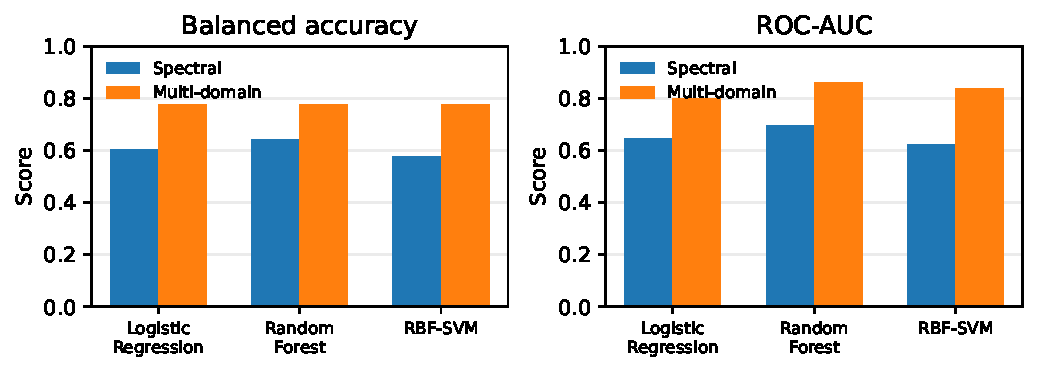
\includegraphics[width=0.96\linewidth]{figures/feature_model_comparison.pdf}
\caption{Balanced accuracy and ROC-AUC for the three learned classifiers under the spectral and multi-domain feature representations.}
\label{fig:comparison}
\end{figure}

The increase from spectral to multi-domain features is consistent across the three classifiers: pooled balanced accuracy rises from 60.3\% to 77.6\% for Logistic Regression, from 64.3\% to 77.7\% for Random Forest, and from 57.6\% to 77.6\% for SVM. Fold-wise balanced accuracy (mean $\pm$ standard deviation) for the spectral representation is 62.93$\pm$3.04\% for Logistic Regression, 67.51$\pm$11.57\% for Random Forest, and 62.58$\pm$4.15\% for SVM. For multi-domain features, the corresponding values are 77.54$\pm$7.06\%, 77.09$\pm$6.56\%, and 77.73$\pm$6.90\%. The fold-wise summaries are not identical to pooled out-of-fold metrics because they average five fold-level scores rather than recomputing a metric over all pooled participants.

For multi-domain Random Forest, the participant-level confusion counts implied by the reported sensitivity and specificity are 49/61 ADHD participants correctly identified and 45/60 controls correctly identified (12 false negatives and 15 false positives). Multi-domain SVM identifies more ADHD participants (54/61) but correctly identifies fewer controls (40/60). The Dummy AUC of 0.350 is not interpreted as meaningful discrimination: its prior probabilities are estimated separately in each training fold, so the pooled scores differ by fold and are not a common ranking scale. The constant majority-class decision is more appropriately summarized by its 50.0\% balanced accuracy.

\section{Graduate Depth Analysis}
The main depth analysis is a feature-representation comparison under a common participant-level validation design. It tests whether the additional nonlinear, wavelet, fractal, Hjorth, and connectivity descriptors provide predictive information beyond band powers and spectral ratios. The consistent increase in balanced accuracy across all three candidate models suggests that the richer representation is useful on this dataset. However, the result does not isolate which individual feature family is responsible: the 199-feature set adds several groups simultaneously, and the ANOVA selector then retains 25 features inside each training fold. A future ablation study should add one feature family at a time and assess stability of selected features. The comparison also exposes a sensitivity-specificity trade-off: SVM is more sensitive to ADHD cases, whereas Random Forest has higher specificity and ROC-AUC.

\section{Limitations and Conclusion}
The independent sample contains 121 participants, not 5,621 independent cases. Participants contribute unequal numbers of epochs, so longer recordings contribute more rows to model fitting. GroupKFold prevents participant overlap but does not stratify the class distribution; only five outer folds are available, and there is no external test cohort. The 2-second windows and 1-second gaps are those of the current code, not the 4-second non-overlapping windows described in an earlier project report. The current implementation also lacks a separate filtering and artifact-removal stage. These choices limit generalization and may affect nonlinear and connectivity features. The results support a dataset-specific finding that the 199-feature representation outperforms the 40-feature spectral subset in this experiment, with multi-domain Random Forest obtaining the highest ROC-AUC. They do not establish clinical diagnostic validity or population-level generalization.

\section{Reproducibility and AI-Use Disclosure}
The experiment code and result files are intended to be available at \url{https://github.com/[YOUR-USERNAME]/[YOUR-REPOSITORY]} (replace this placeholder with the published repository URL). The original dataset is available from IEEE DataPort, DOI 10.21227/rzfh-zn36; the notebook used the Kaggle mirror \url{https://www.kaggle.com/datasets/danizo/eeg-dataset-for-adhd}. The repository should contain the feature-extraction and evaluation code, package requirements, this paper source, the metrics JSON/CSV, and instructions for obtaining the dataset; the raw dataset and API credentials must not be committed. Five-fold GroupKFold, participant IDs, the fixed model settings, and the 0.5 participant-level probability threshold define the reported experiment. Generative AI assistance was used for planning, code debugging, and language editing. The author is responsible for verifying the implementation, results, references, and final submission.

\bibliographystyle{plainnat}
\bibliography{references}

\end{document}
